\section*{Cycle 2 Experiment 10}

\section{\Large{Concurrent Time Server application using UDP}}

\subsection{Aim}
\large To implement Concurrent Time Server application using UDP to execute the program at remote server. Client sends a time request to the server, server sends its system time back to the client. Client displays the result.

\subsection{Theory}
UDP (User Datagram Protocol) is primarily for establishing low-latency and loss-tolerating connections between applications on the internet. UDP sends messages, called datagrams, and is considered a best-effort mode of communications. It is considered a connectionless protocol because it doesn’t require a virtual circuit to be established before any data transfer occurs. \\ \\
\textbf{Server} - The server here waits for the client’s time request. When a request is received, the present system time of the server is sent to the client.\\ \\
\textbf{Client} - The client sends the server a time request. The response from the server is received and provided as the output.
\subsection{Algorithm}
\begin{verbatim}
Algorithm for the Client

1 START
2 Create the socket using socket()
3 Configure socket details
4 Connect the socket to server using function connect()
5 Receive the response from server using recvfrom()
6 Send the acknowledge message to the server using sendto()
7 Print the response
8 STOP

Algorithm for the Server

1 START
2 We can use some time function to return the time
3 Create the UDP socket
4 Configure socket details
5 Bind the address struct to the socket using bind()
6 Receive from client using recvfrom()
7 Send the time to the client
8 STOP
\end{verbatim}

\subsection{Program \& Output}
\begin{verbatim}
//Concurrent time server application using UDP
//Client side
#include <netinet/in.h>
#include <stdio.h>
#include <stdlib.h>
#include <string.h>
#include <sys/socket.h>
#include <sys/types.h>
#include <arpa/inet.h>

#define PORT 4444

int main(){
    char buffer[100];
    char *message = "Concurrent Time Server Application runs successfully!\n";

    int clientSocket, n;
    struct sockaddr_in servaddr;

    bzero(&servaddr, sizeof(servaddr));

    servaddr.sin_family = AF_INET;
    servaddr.sin_port = htons(PORT);
    servaddr.sin_addr.s_addr = inet_addr("127.0.0.1");

    clientSocket = socket(AF_INET, SOCK_DGRAM, 0);

    if (connect(clientSocket, (struct sockaddr *)&servaddr, 
        sizeof(servaddr)) == -1){
        printf("Error in connection.\n");
        exit(0);
    }

    sendto(clientSocket, message, 1000, 0, (struct sockaddr *)&servaddr, 
        sizeof(servaddr));

    recvfrom(clientSocket, buffer, sizeof(buffer), 0, (struct sockaddr *)NULL, 
        NULL);
        
    puts(buffer);

    close(clientSocket);
}

//Server side
#include <stdio.h>
#include <stdlib.h>
#include <string.h>
#include <arpa/inet.h>
#include <sys/types.h>
#include <sys/socket.h>
#include <netinet/in.h>
#include <time.h>

#define PORT 4444

int main()
{
    time_t t;
    time(&t);
    char buffer[100];
    char *message = ctime(&t);

    int serverSocket, len;
    struct sockaddr_in servaddr, cliaddr;

    bzero(&servaddr, sizeof(servaddr));
    serverSocket = socket(AF_INET, SOCK_DGRAM, 0);

    servaddr.sin_addr.s_addr = htonl(INADDR_ANY);
    servaddr.sin_port = htons(PORT);
    servaddr.sin_family = AF_INET;

    bind(serverSocket, (struct sockaddr *)&servaddr, sizeof(servaddr));

    len = sizeof(cliaddr);
    int n = recvfrom(serverSocket, buffer, sizeof(buffer), 0, 
        (struct sockaddr *)&cliaddr, &len);

    buffer[n] = '\0';
    puts(buffer);

    sendto(serverSocket, message, 1000, 0, (struct sockaddr *)&cliaddr, len);
}
\end{verbatim}

\subsection{Output}
\begin{figure}[h]
            \centering
            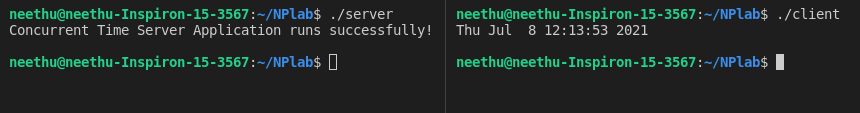
\includegraphics[scale=0.56]{img/exp10.png}
\end{figure}

\subsection{Result}
Implemented the program for the concurrent time server application using UDP using C language in Ubuntu 20.04 with kernel and the above outputs were obtained.

